\chapter{Core Concepts and State of the Art}

The consensus mechanism is a critical component of any blockchain network. It determines the rules of the system, like validating transactions and adding them to the ledger. In order to understand the current development and innovation in this area, it is important to have a solid understanding of the core concepts of blockchains as well as the current state of the art in consensus algorithms. This chapter aims to provide an overview of both of these key topics.

\section{Core Concepts}
This section focuses on the fundamental building blocks of decentralized systems like block\-chains.

This section covers State Machine Replication (SMR), Blockchain Data Structure and Networks, Network Models, and the Concept of Consensus.
Understanding these concepts is crucial for understanding how blockchains networks function in their core, the different trade-offs and design considerations involved in creating and operating a blockchain network. The section starts with an overview of SMR and how it provides consistency and availability in decentralized systems.
Then, the concept of Blockchain Data Structure and its application in decentralized networks is explored. The different Network Models in distributed systems, such as synchronous, asynchronous, and partially-synchronous are also discussed. Finally, the section concludes with a exploration of the topic of consensus and it's importance in blockchain networks.


\subsection*{\textbf{State Machine Replication}}
State Machine Replication is the concept of replicating data in a distributed system, where nodes in a system maintain the same state of a machine. That is, where multiple entities maintain the same information.

In this approach, a node broadcasts an update to its state using a total order broadcast, and all other nodes receive the same updates in the same order and apply it to their own state.

\textbf{Total order broadcast} refers to notion of broadcasting messages in a specific order, such that all nodes in the network receive the messages in the same order, even if the messages are sent from different nodes at different times.

The main advantages of using SMR, like mentioned before, are that it can provide both \textbf{consistency} and \textbf{availability} (in some cases it only provides availability), making it a popular choice for use in blockchain technology, databases, file systems, and other decentralized systems.

Consistency, because it guarantees that every node contains the same state of the machine (not necessarily at the same time), and availability is also ensured because, in case of a node failure, there are other nodes in the system that have the information.

Overall, the concept of State Machine Replication is a fundamental component of decentralized systems that plays a crucial role in ensuring the consistency and availability of shared data. In case of Blockchains, to ensure that every node has the same chain and that there's no single point of failure of the whole system. This makes Blockchain Networks reliable, since in case multiple nodes fail in the network, it can still operate, and that no single node has the power over the whole information, making the network decentralized. 


\subsection*{\textbf{Blockchain Data Structure and Networks}}
Blockchain is a data structure made of blocks that is often compared to a linked list (to which blocks are the nodes of the list), that are connected to a previous block in the chain by a refernce to it, where usually is the hash of the block it is pointing to.

That is, every block, except for the first block (also called ``Genesis'' block), contains the hash of it's previous (or parent) block.

Once a block is added to the blockchain, it cannot be altered or deleted, making the ledger tamper-resistant and immutable, since, in order to change a block's information, one would need to change every child's block hash.
It's also possible to say that, the older the block, the more ``immutable'' it is, or the bigger the number of child blocks a block has, the harder is the tampering of such block. That is because the hash of a block depends on the hash of the previous block, and so on.

Figure \ref{fig:blockchain} illustrates the blockchain datastructure, where it's to possible to observe that the last block (Block N) points to it's parent, and so on. This data structure is often separated by two parts, the header of the block, that contains it's metadata, such as the previous block hash, and the data part, where, in most blockchain networks, this data is where the transactions are stored and visible to everyone that has access to it.

\begin{figure}[H]
    \centering
    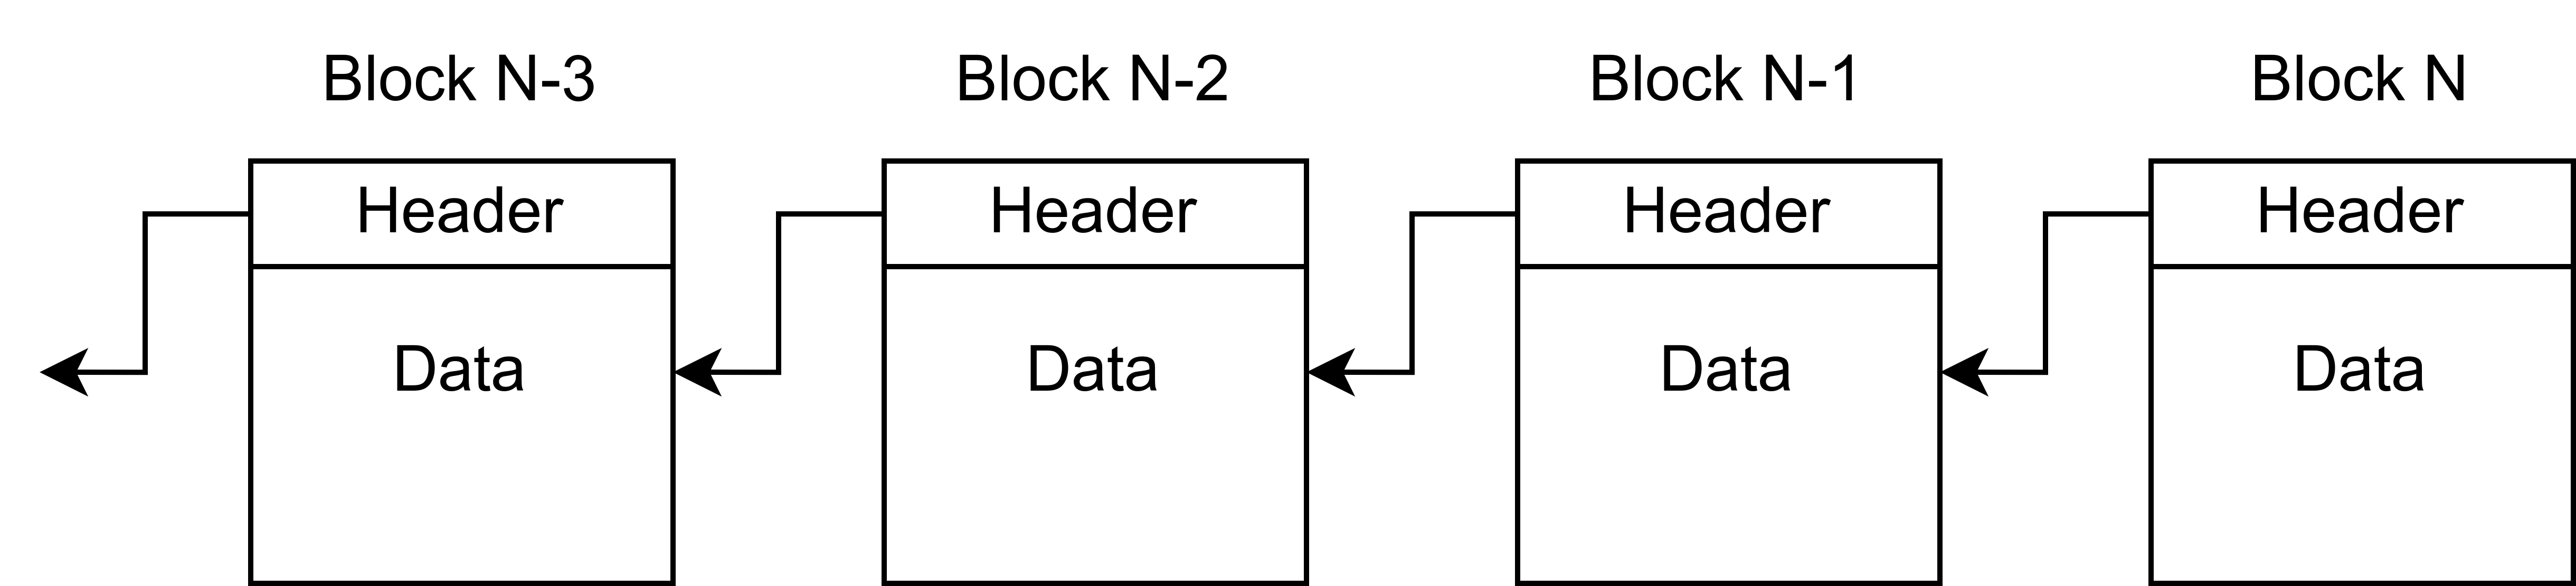
\includegraphics[width=\textwidth,keepaspectratio]{imagens/blockchain.png}
    \caption{Blockchain Datastructure.}
    \label{fig:blockchain}

\end{figure}

Since it is used to record transactions, a blockchain can be considered a ``ledger'', and it's transparent, as all transactions are recorded.

There are networks, like Bitcoin \cite{nakamoto2008bitcoin} and Ethereum \cite{ethereum_foundation} that store and replicate the blockchain (where the chain is the State Machine), with no central authority or entity controlling the network, like mentioned in the previous section. This makes the state of the blockchain highly available, since there are multiple nodes that contain it's information. 

The network reaches ``common consent/decision'' on the contents of a new block through the use of consensus mechanisms, such as Proof of Work or Proof of Stake, which will be described in the next section (\ref{stateoftheart}).
The blockchain is then a distributed ledger, as all nodes in the network have a copy of the ledger, ensuring availability of the state.

The blockchain can be considered the state of a machine, where multiple copies of the state of this machine are stored in multiple nodes, and newer states, that is, the process of appending a new block to the chain, are replicated to every machine in the network.

Beyond cryptocurrency, blockchains have a wide range of potential applications in various industries, like supply chain management, voting systems, and identity verification. The transparent nature of blockchains ensures that all transactions are publicly accessible and verifiable. 

In conclusion, blockchain is a data structure that leverages the concepts of state machine replication to provide availability, leverages the concepts of cryptographic concepts to make it secure, immutable and tamper-resistant ledger where all transactions are recorded, making it transparent.
The decentralized nature of blockchains networks and the use of consensus mechanisms ensure that all nodes in the network have the same state of the chain, providing the availability to access of this information.

\subsection*{\textbf{Network Models}}

The concept of network types is a fundamental aspect of distributed systems and plays a crucial role in their design and implementation of these systems. There are three main models of networks in distributed systems: synchronous, asynchronous, and partially-synchronous. Each has different properties and characteristics that affect the behavior of distributed algorithms and protocols, and it is important to understand these differences in order to design effective and efficient systems.

\textbf{Synchronous networks} are characterized by the fact that the entities in it have a common notion of time and upper bounds on message delay. 
That is, in the Synchronous model, a finite time limit $\Delta$ is established and known. 
The adversary can only delay the delivery of a message sent by at most $\Delta$ time.
This means that the network can guarantee that messages will be delivered within a certain amount of time and that all nodes in the network have a consistent view of the current time. This type of network is relevant when strict timing constraints are necessary, such as in real-time systems.

\textbf{Asynchronous networks} \cite{bracha1985asynchronous}, on the other hand, neither have a common notion of time nor guarantee upper bounds on message delay. 
In this type of network, messages may be delayed indefinitely, and nodes in the network may have a different view of the current time. Asynchronous networks are relevant when timing constraints are not strict. The unpredictability of message delays makes asynchronous networks more challenging to design and implement, but they are also more robust and can handle failures and network partitions more effectively.

\textbf{Partially-synchronous networks} \cite{dwork1988consensus} are a hybrid of synchronous and asynchronous models.
They have a common notion of time but only provide partial guarantees on message delay. In this type of network, some messages may be delivered within a certain amount of time, while others may be delayed indefinitely. Partially-synchronous networks are relevant in scenarios where some timing constraints are necessary, but not all and is often used in blockchain systems, such as Tendermint \cite{buchman2016tendermint}(used in Cosmos Network\cite{tendermintinc} and others), and Tezo's blockchain take on this protocol, Tenderbake \cite{acstefanoaei2020tenderbake}, which balance the need for speed and reliability with the need for resilience and robustness.

In conclusion, the concept of network types is critical in the design and implementation of distributed systems. Understanding the differences between the three networks can help protocol designers make informed decisions about the type of network that best suits their needs and can ensure the success of their systems.

\subsection*{\textbf{Consensus}}
Consensus in Distributed Systems refers to the process of achieving agreement/common consent among all participants in a network on the state of a shared information.

While State Machine Replication is the notion of broadcasting the update of a state and multiple entities maintaining a copy of it, consensus is the concept of how the nodes replicate and decide on a replicated value.

One way to implement total order broadcast, is by sending messages via a designated leader node, but if that leader becomes unavailable, the approach fails. 

So, nodes have to reach an agreement together, in a decentralized manner, on what is the next state of the replicated machine (or who's going decide that next state), and should not be decided by a single node.

Consensus protocols are \textbf{critical} to the blockchain context because they are the mechanisms that allow the network participants to agree on the state of the distributed ledger. In this type of network, transactions are submitted and processed by nodes in a decentralized manner, and the consensus protocol ensures that all nodes have the same view of the ledger and agree on which transactions are valid and should be included in the next state.
The construction of a block is used to make the system more efficient, by ``packaging'' multiple transactions together, but it's possible to reduce this idea to a single transaction being the update to the state.
Also, the algorithms enable the selection of the next leader, that is, the node that takes the transactions, builds the block and broadcasts it to the networks. 

This is important for maintaining the integrity and reliability of the blockchain, as well as for enabling trust in the network among participants who may not necessarily trust each other. A well-designed consensus protocol is essential for ensuring that the blockchain is able to process transactions efficiently and securely, even in the face of network failures, attacks, or other challenges.




\subsection*{Theorems}
There are several important theorems related to consensus algorithms that are relevant to the context of Blockchain Networks, as these are used to attribute characteristics and properties to this type of networks (not only), which include the \textbf{FLP} Theorem \cite{fischer1985impossibility} and the \textbf{CAP} Theorem \cite{brewer2000towards}.


The \textbf{FLP} Theorem states that, in an asynchronous network where messages may be delayed but not lost, it is impossible to achieve both agreement and termination in the presence of process failures. In other words, it's only possible to guarantee two of the following properties at the same time:
\begin{itemize}
    \item Finality or Agreement, that is, if (functioning) have to decide on a value, they all decide one specific one.
    \item Fault Tolerance or Integrity, the system still functions in case of node failures.
    \item Termination or Liveness, where all the functioning nodes decide on value.
\end{itemize}



On the other hand, the \textbf{CAP} Theorem states that, in an asynchronous network where messages may be lost, it is impossible for a distributed system to simultaneously provide the following:
\begin{itemize}
    \item Consistency - all nodes see the same data at the same time
    \item Availability - every request receives a response, without guarantee that it contains the most recent version of the data
    \item Partition Tolerance - the system continues to operate despite arbitrary partitioning due to network failures.
\end{itemize}

Figure \ref{fig:theorems} illustrates these theorems/propreties, where it's possible to observe that the area where the 3 parts meet it's impossible to achieve.

\begin{figure}[H]
    \centering
    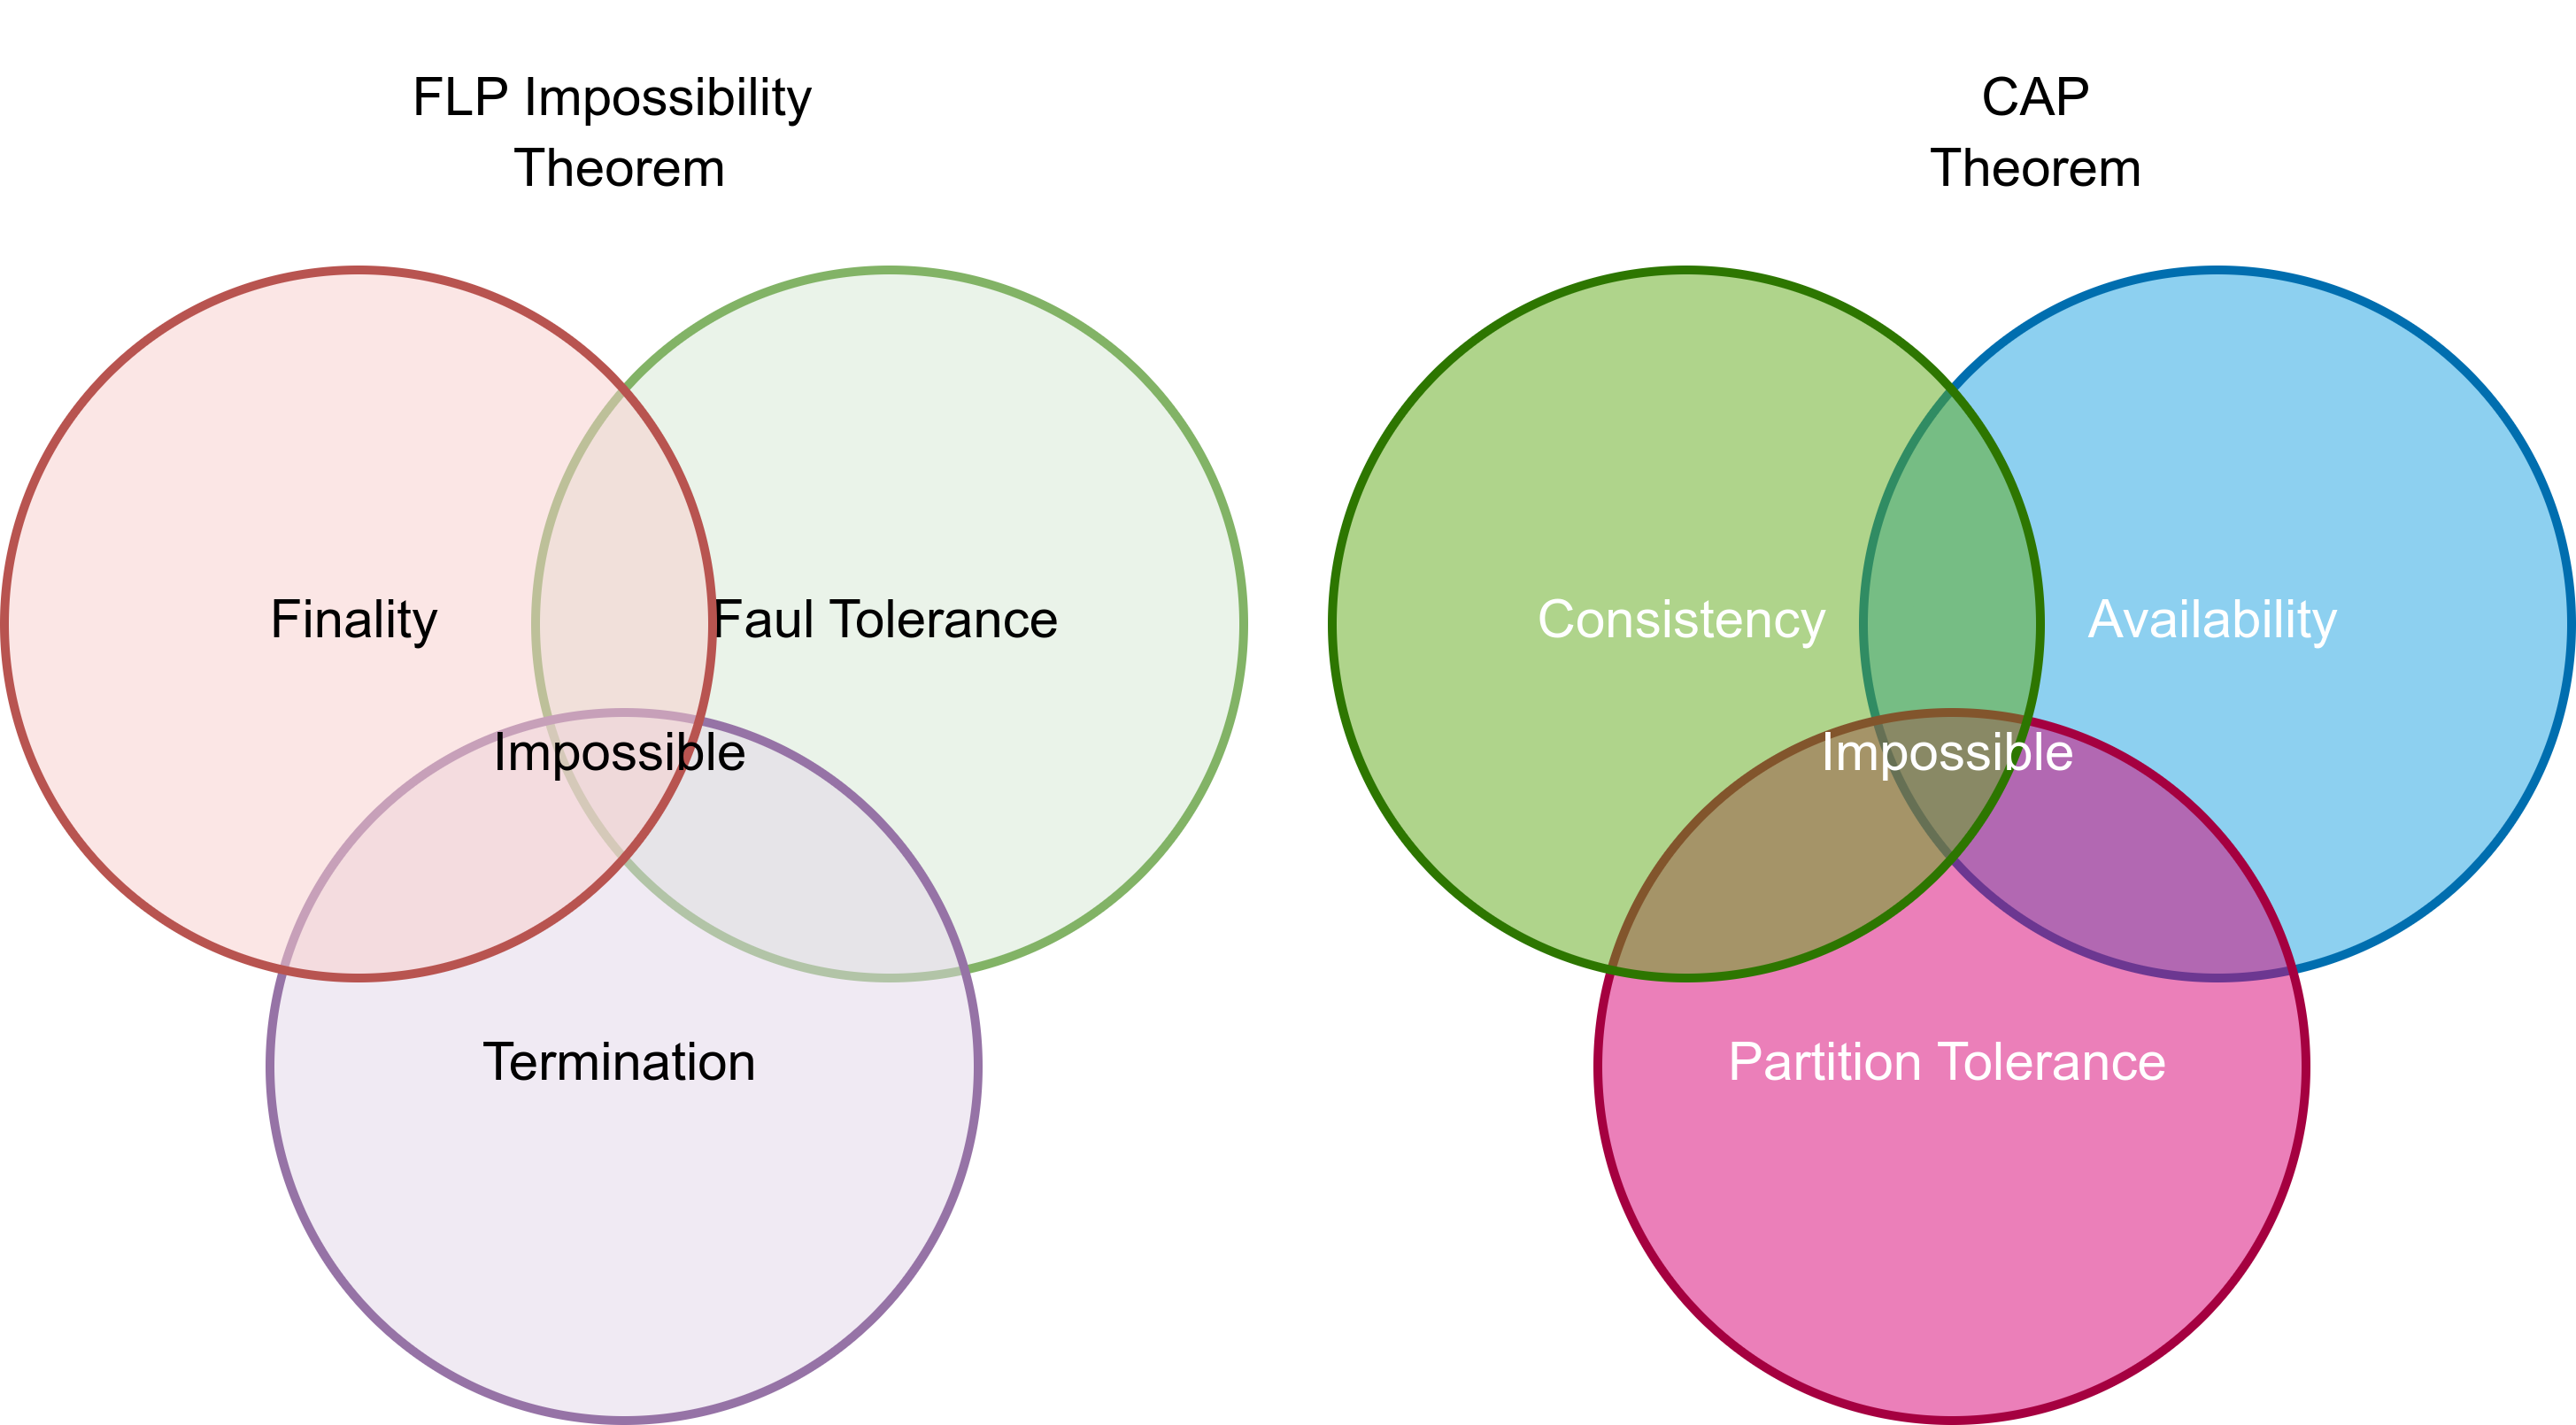
\includegraphics[width=\textwidth,keepaspectratio]{imagens/flp-and-cap.png}
    \caption{FLP and CAP theorems visualized}
    \label{fig:theorems}

\end{figure}



These (and other) theorems provide limits and trade-offs in decentralized systems, and serve as a useful reference for designers and researchers in the field.
In the following sections, more insight about these properties will be provided and why they are relevant to the topic of Blockchain networks, such as the fact that networks like Bitcoin chooses Availability over Consistency (while being Partition Tolerant) and chooses Termination over Finality (while being Fault Tolerant and having a Probabilistic Finality).

\subsection*{Permissioned and Permissionless Blockchains}

Blockchains are a type of decentralized system that uses consensus algorithms to maintain the integrity of its data. In the context of blockchains, the terms ``permissionless'' and ``permissioned'' refer to the way in which participants in the network are allowed to participate in the validation of transactions and the creation of new blocks.
These terms are critical in understanding the trade-offs between security, scalability, and decentralization in blockchains. In this section, we will delve deeper into what ``permissionless'' and ``permissioned'' mean and the advantages and disadvantages of each approach.

\textbf{Permissionless blockchains}, also known as public blockchains, are open to anyone and anyone can participate as a node. No central authority or entity is in control, making it a completely decentralized system. Permissionless blockchains are the most popular type of network and are most often used for cryptocurrencies such as Bitcoin, Tezos and others, where anyone can participate in the network and validate transactions, contributing to the security and reliability of the network.

\textbf{Permissioned blockchains}, are restricted to a set of trusted participants. Only approved entities are allowed to participate as nodes and validate transactions, making it a partially decentralized system. This type of blockchain is often used in business environments where the participants are known and trusted. Usually this networks are faster and more secure (yet, lack decentralization), since the number of participating nodes is way smaller and the fact that nodes are ``handpicked'', they are already trusted.

Known examples are Hyperledger-Fabric \cite{androulaki2018hyperledger}, an enterprise-grade network and Binance Smart Chain \cite{bnb-chain_2022}, a cryptocurrency network that's a fork of Ethereum.

\subsection*{Processes of Block creation}
In the context of blockchain networks, there's a need for nodes selecting the next update to the state, or the next block to add to the blockchain structure. At each round/heartbeat of the network, a proposer decides on the structure of the block (in a cryptocurrency blockchain, the proposer selects the transactions to include in the block).

In this subsection, we will explore the two main ways of reaching consensus/selecting a leader in blockchain networks: proof-based consensus and committee-based consensus.

\textbf{Proof-based consensus} protocols rely on the concept of proof of leadership. Nodes are selected to generate new blocks through a cryptographic random algorithm. The selection of the new leader/proposer is similar to the idea of a lottery. The node that wins such lottery has the right to propose a new block.
Nodes validate transactions, generate a Merkle Tree Root of these, and package them into a new block. The leader node broadcasts the new block and its proof of leadership to the network, that validates the new block, and upon validation, it appends it to the blockchain.


In \textbf{committee-based consensus} protocols, nodes vote to decide the next block to be appended to the blockchain. The proposer multicasts a preparation block request to other participants, who reply with their status. If the proposer receives a sufficient number of ready messages, it enters the pre-commit phase. Participants then broadcast their votes to commit the proposed block. If the number of commit responses agreeing to the new block exceeds a threshold, the block is appended to the blockchain.

\subsection*{Blockchain ``trilemma''}

Another subject that is usually used to compare different blockchain networks, with much discussion, is the topic of the ``Blockchain trilemma'' \cite{buterin} that refers to the trade-off between scalability, security, and decentralization. 
This topic was first introduced by Ethereum's founder \textit{Vitalik Buterin}.

In other words, it is hard, if not impossible to achieve all these three characteristics at the ``same time'' in a public/permissionless blockchain network:
\begin{itemize}
    \item \textbf{Decentralization}: refers to the distribution of power and decision-making authority across all participants in the network. In blockchain, this means that there is no central authority or single point of control, allowing for a more equal and democratic system.
    \item \textbf{Security}: refers to the robustness and reliability of the network, ensuring that data and transactions are protected from tampering, hacking, or other forms of malicious activity.
    \item \textbf{Scalability}: refers to the ability of the network to handle a growing number of transactions and users, without sacrificing performance or speed.
\end{itemize}

Even though that in the context o distributed systems the topic of decentralization isn't relevant, when talking about blockchain networks it's important, as it's one of the main reasons why people use these systems in the first place.

For example, Bitcoin is a highly decentralized and secure blockchain, as there are many nodes (more than 40 thousand  \cite{bitnodes}, as of the writing of this document), yet lacks on scalability, since the creation of a block takes 10min and a transaction takes about 1 to 1.5 hours to complete/be confirmed \cite{gondek}\label{exampleoftime}.

Therefore, when designing a blockchain network, it is important to understand the trade-offs between scalability, security, and decentralization and to make trade-offs based on the specific goals and requirements of the network.

Figure \ref{fig:trilemma} illustrates this trilemma. It's common to assign blockchain network as a point in the area of this triangle. For example, since Bitcoin is secure and decentralized, yet lacks scalability, one could say that it stands near the line between ``Secure'' and ``Decentralized''.

\begin{figure}[H]
    \centering
    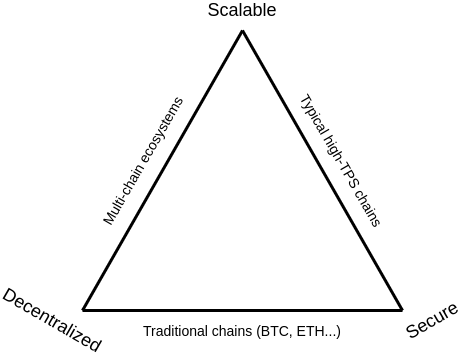
\includegraphics[width=\textwidth/2,keepaspectratio]{imagens/trilemma.png}
    \caption{Blockchain trilemma}
    \label{fig:trilemma}

\end{figure}



\section{State of the Art}
\label{stateoftheart}

In the world of blockchain, consensus algorithms play a crucial role in maintaining the integrity and security of the network. They are the backbone of a blockchain's ability to ensure that all nodes agree on the state of the network, even in the presence of malicious actors, and they are of big importance not only in the matter of ensuring the continuation of the network, but they also play a political and philosophical role in the network.
As blockchain technology continues to evolve, so do the consensus algorithms used to secure them.
Not only they differ on the question of ``Blockchain trilemma'', but each blockchain network has specific characteristics and functionalities that make it unique.

In this State of the Art section, we will delve into the most commonly used consensus algorithms in blockchain technology. We will examine the different strengths and weaknesses of each algorithm and discuss their suitability for different use cases and will also explore milestone and popular protocols.

This will further expose that there's way too many blockchain consensus protocols to choose from when creating a new network.
The reader can obtain additional information about the topics covered in this section at the reference \cite{xu2023survey} and \cite{ferdous2020blockchain}.


\subsection*{\textbf{Proof of Work}}

Proof of work (PoW) \cite{back2002hashcash} was originally introduced as a solution to the problem of spamming and abuse on the Internet. In a proof of work system, a computational problem is designed such that it requires a significant amount of computational effort to solve, but its solution can be easily verified. The idea is that, by requiring a party to perform a certain amount of computational work in order to perform a certain action, such as sending an email or posting a message, the system can ensure that the action is performed in a responsible and controlled manner.

The first use of proof of work was in the context of a system for fighting email spam, designed by computer scientist Adam Back in 1997. In this system, an email sender was required to perform a certain amount of computational work, in the form of solving a cryptographic puzzle, to send an email. The idea was that the cost of performing the work would make it unfeasible for spammers to send large quantities of unsolicited email, while still allowing legitimate users to send email without significant difficulty.


Proof of Work was later adapted as a consensus algorithm used by many blockchain networks, Bitcoin \cite{nakamoto2008bitcoin} being the most popular network to do so.
Bitcoin or ``Nakamoto Consensus'' was also the first instance of the Proof of Work Consensus and of a blockchain network.

The idea behind PoW (applied to blockchain networks) is that, in order for a block (containing a list of transactions) to be added to the blockchain (and replicated), at least one node in the network has to package together a list of transactions into a block and solve a cryptographic hard problem in order for it to be valid.
That is, the block has to contain a stamp or a proof that actual computational work was put in to create a block.
That work/computational power is provided by nodes called ``miners'', and these miners compete to be the first to solve the cryptographic puzzle, where the first to solve it is selected as the leader and has the ability to add the their created block to the blockchain.

In a permissionless environment, it's complex to make a democratic system where each entity could cast a vote, since a malicious entity could create many fake identities or nodes to manipulate the network, known as a ``sybil attack''.
In blockchain networks, entities make use of Public-key cryptography to be identified, so a malicious entity could create as many pairs of Public-Private keys as it wished to cast as many votes as it wanted.

The ``Nakamoto Consensus'' (where PoW is used) was the first to be tolerant to sybil attacks in a permissionless setting.
It prevents these attacks by making it computationally expensive for an attacker to try to disrupt the network, since, instead of voting power being concentrated on the number of votes for an election, it's replaced by the idea of computational power, where an attacker would have to do as much work as the rest of the network (assuming that it's not malicious) in order to gain a majority, and that could imply problems to the malicious entity, like large electricity costs in case of mining.
By requiring a significant amount of computational power to mine blocks, PoW ensures that only legitimate nodes with real computational resources will be able to participate in the network.
Mining is what is called coequally to the process of using computational power to solve cryptographic puzzles and adding blocks to the blockchain.

In other words, instead of entities voting for a block to be added to the blockchain, the ``vote'' is done by solving puzzles, where the first to solve such puzzle is the one deciding the block to be added. Another analogy can be that the winner of the ``lottery''  get's the prize of deciding the next block (solving the puzzle is actually a random chance process, where increasing the mining power also increases the chance of winning).

Mining has several purposes in PoW, such as leader selection and preventing sybil attacks, like mentioned before, but also enforcing block timing with difficulty adjustment and, in case of cryptocurrency blockchains, to add new value/mint new currency into the system and rewarding those who do the computational work. 

The difficulty adjustment ensures that the time between blocks is consistent (in Bitcoin, that is 10min), and the computational difficulty to mine new blocks adjusts accordingly. When in a epoch (in Bitcoin, that is 2016 blocks), the median time taken to mine a block was lower than it should've been, the difficulty is increased proportionally to make it harder to mine, so it actually takes the pretended time, and vice versa.

The mining also introduces/mints new currency into the system, since itself doesn't have any value in it initially (it's a closed economic system, no more currency can be put into it), and that currency is awarded to the participants of the mining process.


\subsection*{Properties of Proof of Work Consensus}

The properties of PoW consensus can be analyzed through the FLP theorem and the CAP theorem, which were discussed in the previous section.

Regarding the FLP theorem, PoW exhibits Probabilistic Finality \cite{anceaume2020finality}. This means that all functioning nodes eventually agree on a single block, but the process is not deterministic and involves a certain degree of probability. The waiting for confirmations adds an additional layer of security to the consensus process. Like mentioned before in this example (\ref{exampleoftime}) in Bitcoin this takes about 6 confirmations, or about 1 hour, since a block usually takes 10 minutes to created. This happens because mining is a process independent from the state of the network and independent from other nodes, and two or more nodes can solve the cryptographic puzzle/build a block ``at the same time'' (until the whole network agrees on the same block).
When this happens, a node can receive more than one valid candidate extending the same chain, and each protocol handles this in a specific way. This is what is called a ``Fork''.
Once again, taking Bitcoin as an example, a node handles this case by using the rule of the longest chain (Longest Chain Rule), where, when a node has two competing blocks, where each makes a branch, it waits until one of the branch is bigger than the other.
This is done because, the branch with the most computational power is the one with the bigger chance of being extended.

PoW also demonstrates Fault Tolerance, making it a form of Byzantine Fault Tolerance (BFT). This is achieved through the complex and expensive mining process, which makes it economically infeasible for a malicious node to alter the data in a block and catch up with the rest of the network. The incentive to follow the longest blockchain also adds to the fault tolerance of the consensus mechanism.

Finally, PoW also exhibits Termination, meaning that every functioning node reaches a decision, even if it's not the final one (because of the Probabilistic Finality). 

Regarding the CAP theorem, PoW may not provide Consistent results, as a node might not have the latest block when requested, and like mentioned before, forks can happen, and so different nodes can contain different chains (for a period).
However, it does provide Availability, as miners are continuously trying to mine new blocks, the difficulty level of mining is adjusted to ensure the steady addition of blocks to the blockchain and there are multiple nodes in the network.
PoW is also Partition Tolerant, meaning that even if a portion of the nodes stop functioning or the network splits, the blockchain can still function and recover.

\subsection*{Nakamoto Consensus}
In the previous subsection, we discussed the consensus mechanism used in blockchain technology where participants in the network compete to solve complex mathematical puzzles in order to validate transactions and generate new blocks.
We introduced the concept of miners, who play a crucial role in this process, and how they are incentivized through rewards for their efforts.

Building on this foundation, we now delve into the specifics of the Nakamoto Consensus, named after the pseudonym used by the unknown creator(s) of Bitcoin (Satoshi Nakamoto). The Nakamoto Consensus is a milestone in the history of blockchain technology and a major innovation in the field of consensus algorithms.

The Bitcoin network is a Peer-to-Peer network, where blocks and transactions are gossiped by the nodes and where they are also responsible for generating blocks, just like mentioned previously.

This acts as a barrier to entry for malicious actors, as it becomes extremely difficult for them to launch Sybil attacks by generating many fake nodes.
The puzzle in Bitcoin involves computing a nonce (basically, a number) that meets certain conditions, as outlined by the equation $H(hi−1,nonce,tx,par) < Target$, where ``hi−1'' is the hash of the previous block, ``tx'' represents the set of validated transactions, and `'par'' represents other parameters such as blockchain version and cryptographic parameters, and the ``Target'' is a value decided by the network (that encoded the current difficulty).

The usual workflow of a node is the following:
\begin{itemize}
    \item Node gossip transactions in the network (They are temporally stored in a data structure that is called ``Mempool'').
    \item When a node receives a block from the network, it appends it to it's own blockchain stored.
    \item To start the mining process, a node selects multiple transactions for the transaction part of the block. There's a size limit in bytes for this part, and the selection criteria is irrelevant, they only have to be valid.
    \item It creates a new block header with information, like, the hash of the previous block, a nonce (a integer number) and a Merkle Tree Root Hash of the transactions and other information (that is irrelevant to this).
    \item The node tries out every possible value for the nonce until the resulting hash (SHA256 hash function) of the header has a value bellow the current target.
    \item If a node receives a new block from the network before it finds itself the nonce, it stops the mining and appends such block. If it finds the nonce, it shares the block with the network and it's rewarded.
    
\end{itemize}

When a entity creates a transactions, it can also offer a fee. This is used to prevent transactions spamming and also acts as a ``place in the block'' auction.
Besides block creation reward, the miner also receives these transactions fees, so miners will select transactions based on that fee, and other attributes of the transactions.

The difficulty/target of the puzzle is adjusted periodically (every 2016 blocks like mentioned before), depending on the actual block generation intervals and the expected block generation intervals (of around ten minutes in Bitcoin). 
This allows Bitcoin to maintain a consistent block generation time of around ten minutes, regardless of the computational power in the network.

\subsection*{Improving Proof of Work}

The Nakamoto Consensus protocol, despite being the first consensus mechanism for block\-chains and widely adopted, has limitations when it comes to scalability, security, and decentralization.

There are multiple ways of improving the Nakamoto Consensus protocol, and doing so has resulted in the creation of new blockchain networks. These changes move the consensus protocol within the triangle formed by the ``trilemma'', but they also come with new challenges compared to the original consensus for blockchains.

This topic is relevant to this thesis since it's these characteristics that differentiate consensus even further.

\subsection*{Improving Scalability}
Blockchain networks have faced scalability issues since their inception. A consensus mechanism must maintain security and decentralization, so it's challenging to scale the network and improve the transaction processing speed. To overcome this challenge, several solutions have been proposed, including decoupling blockchain functions, parallel chains, and DAG-based protocols.

\textbf{Decoupling of Blockchain Functions}: The functions of blocks in a blockchain network can be separated into key blocks for leader election and microblocks for transaction packing. By doing so, the miner who successfully solves the puzzle becomes the leader of an epoch and generates key blocks and microblocks. This method helps to improve the throughput of the network, but it doesn't significantly reduce the transaction confirmation latency. Also, it comes with problems such as the fact that the leader can be compromised during the epoch.

\textbf{Parallel Chains}: The parallel chains method involves miners extending parallel chains simultaneously to improve the blockchain throughput. In this method, miners compete to solve puzzles, and the generated block is appended to one of the chains based on the random hash value of the puzzle solution. While this improves throughput, a malicious entity could still target a single chain.

\textbf{DAG-based Protocols}: instead of using a traditional blockchain structure, DAG-based protocols utilize a tree-like structure, called a Directed Acyclic Graph (DAG). The DAG structure allows for concurrent block generation and operates differently than blockchain structures. Unlike parallel-chain protocols that have multiple independent genesis blocks at initialization, there is only one genesis block in DAG-based protocols. If the DAG-based block\-chain follows the longest chain rule, there will only be one longest chain, instead of multiple chains in the parallel-chain scheme, and blocks on the forks will be pruned. This structure provides a unique approach to improving scalability in blockchain networks 

\subsection*{Improving Security}
Blockchain networks are vulnerable to various security attacks, such as selfish mining attacks \cite{grunspan2018profitability} and double-spending attacks \cite{chaudhary2020double}.
To improve the security of blockchain networks, various solutions have been proposed, including changing the incentive mechanism in the chain and how it's shared.

The FruitChain \cite{pass2017fruitchains} protocol is a blockchain protocol that improves on this while still providing the same consistency and liveness properties as Nakamoto consensus. 
With FruitChain, any honest set of nodes controlling a certain fraction of computational power is guaranteed to get at least that fraction of the block generation and rewards in any length segment of the chain, making it harder for coalitions between miners to happen.

\subsection*{Improving Decentralization}
To improve decentralization, several solutions have been proposed,
including de-incentivizing centralized activities 
like pool mining and incentivizing decentralized/solo mining using methods like eradicating ASIC (Application-Specific Integrated Circuits) mining.

Pool mining is a point of centralization in Proof of Work networks. The idea of pool mining is that there's a single node (connected in the network) that communicates with multiple miners, that is, entities which their only purpose is to find a nonce.
These miners join to mine a single block as if they were only a single node, so they have more computational power together, and inherently having a bigger change of finding a block. When a block if found by the pool (a node, as viewed from the network), the reward is shared with all the miners, depending on how much effort they put into the mining.
The problem comes with the fact that most mining nowadays, like in Bitcoin, is done by groups like this, and so, the owners of these pool nodes have a lot of power over the network, as they can make decisions on the block creation, like black-listing transactions from someone, or selecting transactions based on unfair criteria.

Also, with the increase of hashing power, that is, the computational power of blockchains, miners have improved the mining process by developing highly specialized hardware, called ASICs.

By doing so, it's infeasible for anyone (without this type of hardware) to join the mining process, and centralizing the power on the owners of ASICs and the it's manufacturers. So there are multiple efforts to erradicate this type of mining like by using memory-hard puzzles, that are harder for ASIC hardware than for Personal Computer Hardware (like GPUs or CPUs), or using hash functions that are hard to implement as ASICs.

This is the case of Monero \cite{getmonero.org}, that besides providing total privacy (the ledger isn't transparent like bitcoin), is also designed to promote equality between miners by using an egalitarian approach based on the use of a different hash function (compared to Bitcoin, that uses SHA256) called ``CryptoNight'', which is said to be memory-hard, making it hard for the development of ASIC hardware and also hard for mining using GPUs. 

\subsection*{\textbf{Proof of Stake and Its Variants}}
Proof of Stake (PoS) has emerged as a popular alternative to Proof of Work (PoW). In PoS, nodes are selected to validate transactions and create new blocks based on their stake in the network. The core idea is similar to PoW but replaces "computational power" with "stake," making it more energy-efficient \cite{reference_needed}.

\textbf{Chain-based Proof of Stake (ChainPoS)}: Focuses on incentivizing stakeholders to act honestly by staking assets. It offers two main approaches for block creator selection: randomized stakeholder selection and a hybrid between PoW-like selection and randomized stakeholder selection. Peercoin \cite{peercoin_foundation} and Casper FFG \cite{buterin2017casper} are notable examples.

\textbf{BFT Proof of Stake (BFT PoS)}: Developed to tackle Byzantine faults in decentralized systems. It operates in a multi-round consensus process involving validator selection and the use of quorums of super-majority. Tendermint and Tenderbake in the Tezos blockchain are examples \cite{lamport2019byzantine}.

\textbf{Delegated Proof of Stake (DPoS)}: Combines elements of PoS and democratic governance. It aims to balance decentralization with efficiency by having a smaller number of delegates. Validators are selected based on reputation scores or other metrics, and stakeholders can vote for delegates.

In conclusion, PoS and its variants offer a range of options that balance security, scalability, and efficiency, each with its own set of trade-offs and benefits.

\subsection*{\textbf{Proof of Authority and Its Variants}}
Proof of Authority (PoA) is a consensus algorithm commonly used in permissioned blockchain networks, where decentralization is not the primary concern. In PoA, a limited set of pre-approved validators are responsible for block creation and transaction validation. This approach offers a high degree of efficiency and scalability while eliminating the need for resource-intensive calculations.
Interestingly, we also implemented a PoA, that has certain similarities with PoW, a topic that will be explored further in this document.

\textbf{Clique PoA}: This variant aims to improve the decentralization aspect of PoA by allowing multiple authorities to propose blocks in a round-robin manner. This reduces the risk of a single point of failure and enhances network security \cite{szilagyi2017clique}.

\textbf{Aura PoA}: Known for its flexibility, it allows validators to take turns in a defined order to create blocks. It also includes a mechanism for validators to communicate and come to a consensus if a block is valid or not \cite{aura_poa}.

\textbf{IBFT PoA (Istanbul BFT)}: A Byzantine-fault-tolerant PoA algorithm that can handle malicious nodes and network splits. It uses a voting mechanism among validators to reach consensus and is known for its robustness \cite{moniz2020istanbul}.

In conclusion, PoA serves as an effective choice for networks where rapid transaction validation is crucial, and where a permissioned structure is acceptable. Its variants offer different ways to balance efficiency with security, making PoA adaptable to various specific needs.


\subsection*{\textbf{Other Consensus Protocols}}

Apart from Proof of Work and Proof of Stake, there are other consensus algorithms that are used in the blockchain industry. However, they are not as popular as PoW and PoS and are mainly used in niche applications or not used in the popular cryptocurrency blockchains. In this section, we will explore and explain some of these alternative consensus algorithms.

In this subsection we will enumerate and give a overview of a few of these consensus algorithms.

\textbf{Proof of Burn} \cite{karantias2020proof} shares some characteristics with Chain-based Proof of Stake. In this algorithm, instead of staking, the node sends some tokens to an address that is difficult to access, essentially "burning" them. The node can then mine or validate blocks proportionate to the amount of tokens that were burned. The idea behind Proof of Burn is that a node is willing to sacrifice tokens, making it less likely that they would act maliciously as they would lose their investment.

\textbf{Proof of Research} \cite{gridcoin} algorithm is used in some cryptocurrencies that aim to provide an environmentally friendly alternative to Proof of Work. In this algorithm, nodes perform research tasks that can range from solving mathematical problems to annotating data. The first node to complete the task is allowed to mine the block, providing a solution to the computational waste that is inherent in PoW.

\textbf{Proof of Capacity/Space/Storage} \cite{dziembowski2015proofs} shares some characteristics with Proof of Work. In this algorithm, nodes are required to dedicate a certain amount of disk space for storage. The more disk space a node dedicates, the more chances it has of being selected to mine the next block. The algorithm is energy-efficient compared to PoW, but it still suffers from centralization problems as nodes with more disk space are more likely to be selected to mine blocks. These kinds of protocols are often used in conjunction with other blockchain networks (Proof of Work or Proof of Stake) to store large amounts of information that wouldn't be feasible to store directly in those blockchains.

\textbf{Trusted Computing} \cite{bowman2021elapsed} algorithms use the secure hardware provided by Trusted Execution Environments (TEEs) to secure the consensus mechanism. One example of such an algorithm is POET, used in the Hyperledger blockchain platform. In POET, a trusted party generates a wait time for each node and the first node to complete the wait time is allowed to mine the next block. The use of TEEs ensures that the wait time cannot be tampered with, providing a secure mechanism for consensus.

There are many alternative consensus algorithms that are used in the blockchain industry, each with its strengths and weaknesses.
While some, like Proof of Burn and Proof of Research, offer environmentally friendly alternatives, others, like Proof of Capacity/Space/Sto\-rage, offer a totally different concept of proof.
Trusted Computing Algorithms, like POET, provide secure consensus mechanisms, but rely on trusted hardware that may not be readily available and making it more centralized, as it relies on specific companies to build this kind of hardware.
Ultimately, the choice of consensus algorithm will depend on the specific use case and requirements of the blockchain platform.





\subsection*{\textbf{Lupin Language}}
\label{lupin}

The Lupin Language is a Domain-Specific-Language (DSL) that is currently in its early stages of development. 
The process of compilation of this language results in OCaml language code.
It is designed to simplify the process of designing and coding consensus algorithms, which can be a challenging task that requires a significant amount of expertise and resources.

Not only that, but it can also be used to perform rigorous formal analysis and verification on these algorithms, bringing 
a whole new level of capability to analyzing consensus algorithms and will be an important tool in the future.

This project provide will provide feedback for the development of Lupin and may also serve as a layer of execution for the results of its compilation, and is in collaboration with the Lupin Language project and its results will be further exposed in a later section.



\section{Conclusion}
This chapter provides a comprehensive overview of the core concepts of blockchains and the state of the art in consensus algorithms. With so many different consensus protocols available, it is essential to have a clear and concise way to compare and evaluate them. As the field of blockchain continues to evolve, the development of more effective consensus algorithms will be a critical factor in determining the success of blockchain networks. By gaining a deeper understanding of the current state of the art, researchers and developers can work towards developing new consensus algorithms that are more secure, efficient, and scalable than ever before.
